\documentclass[oneside,final,14pt,a4paper]{extreport}



\usepackage[utf8]{inputenc}
%\usepackage[english, russian]{babel}
\usepackage[russianb]{babel} % адаптация русского языка
\usepackage{vmargin} % настройка размера полосы набора
\setpapersize{A4}
\setmarginsrb{2cm}{2cm}{2cm}{2cm}{0pt}{0mm}{0pt}{13mm} % {левое поле}{верхнее поле}{правое поле}{нижнее поле}{колонтитулы}{колонтитулы}{колонтитулы}{номер страницы}
\usepackage{indentfirst} % отделять первую строку раздела абзацным отступом
\usepackage{graphicx} % подключение библиотеки для работы с внешними картинками
\usepackage{setspace} % для изменения межстрочного интервала
\sloppy % выравнивание текста
\setstretch{1.5} % устанавливаем межстрочный интервал

\usepackage {titlesec}
% меняем заголовок для команды \chapter и запрещаем переносы слов
\titleformat{\chapter}{\hyphenpenalty=10000\normalfont\huge\bfseries\flushleft}{\thechapter\space\space}{0pt}{\huge}


%\usepackage[OT1]{fontenc}
%\usepackage{amsmath}
%\usepackage{amsfonts}
%\usepackage{amssymb}
%\usepackage{graphicx}
%\usepackage[left=2cm,right=2cm,top=2cm,bottom=2cm]{geometry}
%\usepackage{cmap} % для кодировки шрифтов в pdf
% \usepackage{indentfirst} % отделять первую строку раздела абзацным отступом


\makeatletter
\renewcommand{\@biblabel}[1]{#1\space} % Заменяем библиографию с [number] на просто number:
\makeatother


\begin{document}





% ТИТУЛЬНЫЙ ЛИСТ НАЧИНАЕТСЯ
\thispagestyle{empty}
\begin{titlepage}

\begin{figure}
	\centering
	
\includegraphics[width=0.5\textwidth]{msu}\\
\end{figure}

\begin{spacing}{1.0} % устанавливаем межстрочный интервал
\begin{center} % центрируем текст
	{\small
		Московский государственный университет имени М.В. Ломоносова \\
		Факультет вычислительной математики и кибернетики \\
		Кафедра автоматизации систем вычислительных комплексов \\
	}
	\vspace{4cm}
	{\large Романов Андрей Романович \\}
	\vspace{1cm}
	{\large\bfseries
		Разработка системы обеспечения надежного и \\
		масштабируемого 	виртуального сетевого сервиса в \\
		облачной среде \\
	}
	\vspace{1cm}
	ВЫПУСКНАЯ КВАЛИФИКАЦИОННАЯ  РАБОТА
\end{center}
\vfill
\begin{flushright}
\begin{small}
	{\bfseries Научный руководитель: \\}
	к.ф.-м.н. \\
	В.А. Антоненко \\
\end{small}
\end{flushright}

\vfill

\centerline{Москва, 2016}
\end{spacing}
\end{titlepage}
% ТИТУЛЬНЫЙ ЛИСТ ЗАКАНЧИВАЕТСЯ
\setcounter{page}{2}





\chapter*{Аннотация}
В данной работе рассматриваются проблемы организации надежной работы и масштабируемости виртуального сетевого сервиса.

В рамках выпускной квалификационной работы рассмотрен высокоуровневый стандарт архитектуры NFV платформ ETSI NFV MANO. Проанализированы существующие решения, решающие задачи восстановления сервиса и расширения его инфраструктуры.

Разработан программный модуль, интегрированный в облачную платформу Cloud Conductor и полностью соответствующий архитектуре ETSI NFV MANO. Модуль позволяет управлять виртуальными сетевыми сервисами и обеспечивает их отказоустойчивость и масштабируемость автоматическом режиме. Проведены эксперименты, подтверждающие автоматическое восстановление корректной работы сервиса в случае возникновения неполадок или в случае нехватки ресурсов.





% Оглавление
\tableofcontents % генерация оглавления





\chapter*{Введение}
\addcontentsline{toc}{chapter}{Введение} % добавить Введение в оглавление

В современных сетях функционирует огромное количество сервисов: маршрутизация (routing), трансляция сетевых адресов (NAT), сетевой экран (firewall), туннелирование (VPN), проски-сервер и т.д.. Многие из них реализованы в одном физическом устройстве (маршрутизатор). Для эффективной работы сервисов нагрузку распределяют сразу на несколько таких устройств. 

При возникновении необходимости в дополнительных функциях требуется приобретать оборудование, часть функциональности которого будет избыточной. 

Функции, реализованные в составе отдельных сетевых узлов, зачастую плохо масштабируются, так как при увеличении нагрузки на сеть увеличивается число необходимых физических устройств. При обычных (не пиковых) нагрузках часть устройств простаивает. Следовательно, становится актуальным вопрос динамической масштабируемости сервиса в зависимости от его загрузки.

Одной из проблем современных сетей является зависимость от производителя аппаратных устройств. Оборудование разных производителей может конфликтовать между собой. Со временем вендоры перестают поддерживать устаревшие устройства.

Таким образом, можно выделить ключевые проблемы организации работы сетевого сервиса:
\begin{itemize}
	\item использование оборудования с избыточной функциональностью;
	\item рассчет производительности сервиса исходя из максимальной возможной нагрузки;
	\item простаивание оборудования в случае, если нагрузка не является пиковой;
	\item зависимость от производителя оборудования (техническое обслуживание и устаревание оборудования, невозможность модифицировать сервис без вмешательства производителя);
\end{itemize}

Для введения понятия концепции виртуальных сетевых функций нам потребуется рассмотреть существующие модели обслуживания облачных вычислений: 
\begin{itemize}
	\item Infrastructure-as-a-Service (IaaS) -- инфраструктура как услуга;
	\item Platform-as-a-Service (PaaS) --  платформа как услуга;
	\item Software-as-a-Service (SaaS) -- программное обеспечение как услуга;
\end{itemize}

IaaS - модель, в которой клиенту предоставляется возможность использования облачной инфраструктуры. Пользователь сам управляет программным обеспечением предоставленных ему ресурсов. Контроль и управление физическими ресурсами облака осуществляется облачным провайдером.

Paas - модель, в которой клиенту предоставляется возможность использования облачной инфрастуктуры для управления базовым программным обеспечением. В составе таких плафторм присутствуют средства для создания такого программного обеспечения.

SaaS - модель, в которой клиенту предоставляется возможность использования программного обеспечения облачного провайдера. Контроль и управление физическими ресурсами облака и предоставляемого програмного обеспечения осуществляется облачным провайдером. Основное преимущество модели SaaS для потребителя услуги состоит в отсутствии затрат, связанных с установкой, обновлением и поддержкой работоспособности оборудования и работающего на нём программного обеспечения.~\cite{bib:saas}

Концепция виртульных сетевых функций (Network Function Virtualization, NFV) --- это технология, позволяющая виртуализировать сетевые сервисы, которые на данный момент реализованы лишь на физических устройствах. Под виртуализацией сетевых сервисов понимается предоставление сетевых услуг в виде программного обеспечения, функционирующего на одной или нескольких связанных виртуальных машинах. NFV работает в рамках модели SaaS. Свойства концепции NFV:
\begin{itemize}
	\item масштабируемость - в зависимости от загруженности сервиса будет задействована та часть инфраструктуры, которая необходима для корректной работы;
	\item надежность - в случае сбоев в работе сервиса будут предприниматься действия по восстановлению его работы в автоматическом режиме;
	\item гибкость - виртуализация позволяет быстро развертывать сервисы на новой инфраструктуре;
\end{itemize}

Концепция NFV отделяет программную составляющую сетевых функций от аппаратной (вычислительные и сетевые ресурсы). Такой подход подразумевает использование физической инфраструктуры, не зависящей от производителя, что требует стандартизации интерфейсов между различными компонентами системы.

Разработкой высокоуровневой архитектуры ETSI NFV Management and Orchestration (ETSI NFV MANO) для  NFV платформ занимается организация ETSI. Главной особенностью архитектуры является оптимальное использование инфраструктуры: она выделяется для каждой функции по запросу. Базовыми блоками, из которых строятся виртуальные сетевые сервисы, являются виртуальные сетевые функции (VNF). Платформа на базе ETSI NFV MANO умеет размещать VNF на подконтрольной инфраструктуре. В результате комбинирования блоков VNF получаются виртуальные сетевые сервисы (VNS), которыми пользуются клиенты платформы.

Целью данной работы является разработка модуля управления виртуальными сетевыми сервисами. Модуль должен обеспечивать отказоустойчивость и масштабируемость сервисов в автоматическом режиме.

В разделах \ref{sec:nfv_description} и \ref{sec:etsi_nfv_mano} подробно рассматривается концепция NFV и архитектура ETSI NFV MANO. Далее в разделе \ref{nfv_platform_overview} приводится обзор существующих NFV платформ. В разделах \ref{chap:practice} и \ref{chap:expirements} приводится описаниия практической части и экспериментов.

Для исследования разработанного решения были проведены эксперименты, подтверждающие автоматическое срабатывание тригерров для масштабирования инфраструктуры сервисов и восстановление работы сервиса после сбоя.





\chapter{Постановка задачи}
\label{chap:problem_statement}
Целью данной работы является разработка решения, которое управляет жизненным циклом виртуальных сетевых сервисов и обеспечивает их надежную работу и масштабируемость.

Разрабатываемый модуль должен работать в облачной среде. Это означает, что все клиенты виртуальных сетевых сервисов являются виртуальными машинами. Далее под клиентом виртуального сетевого сервиса будем подразумевать виртуальную машину.





\chapter{Обзор предметной области}
\label{chap:overview_subject_area}

\section{Общее описание NFV}
\label{sec:nfv_description}
В 2004 году была предложена идея организации сетевой инфраструктуры с целью снижения затрат и ускорения внедрения новых услуг. Она состояла в объединении ядра сети и сети доступа в единую платформу. Однако без виртуализации идея не получила широкого распространения.\cite{nfv-state2}

NFV предполагает использование виртуализированной инфраструктуры для функционирования услуг. Концепция предлагает использование технологий для виртуализации функций в виде составных элементов, которые могут быть связаны для создания телекоммуникационных сервисов. 

Таким образом, виртуальная сетевая функция (VNF) --- это описание требуемой инфраструктуры, требуемого программного обеспечения, параметров подключения пользователей к это услуге и т.д.. Заметим, что программное обеспечение, описанное в VNF должно иметь ограниченную и законченную функциональность. Не следует виртуализировать сложное программное обеспечение, так как оно будет использовать дополнительные ресурсы инфраструктуры.

Виртуальный сетевой сервис (VNS) - это некоторое множество связанных между собой виртуальных сетевых функций. Это конечная услуга, которая будет предоставляться клиентам. Концепция предполагает внутреннее представление VNS как произвольное непустое множество, состоящее из VNF. При этом VNF как-то связаны друг с другом.

По мнению автора, наиболее интересен случай цепочек виртуальных сетевых функций (VNF chaining). В этом случае можно считать каждую VNS как цепочку сетевых функций. Близкую аналогию можно провести с математическим понятием функции. Пусть $x$ - это входящий трафик некоторого объема. Тогда результатом работы сервиса $S$, состоящего из последовательной цепочки функций $f_{1}$, $f_{2}$, $f_{3}$ будет трафик $y$, такой что:

\begin{equation}
	\label{eq:service_example}
	y = f_3(f_2(f_1(x))) = S(x)
\end{equation}

В результате трафик $x$ трансформировался в трафик $y$. $S$ - это суперпозиция функций $f_{1}$, $f_{2}$, $f_{3}$.


\section{Архитектура ETSI NFV MANO}
\label{sec:etsi_nfv_mano}
Европейский Институт Телекоммуникационных Стандартов (ETSI) в 2013 году опубликовал высокоуровневые рекомендации по разработке платформы, управляющей виртуальными сетевыми сервисами Network Function Virtualization Management and Orchestration (NFV MANO). Основная цель документа --- стандартизировать интерфейсы каждого модуля в платформе.\cite{nfv-mano-state1} Как показано на Рис.~\ref{nfv-mano-image1}, в ETSI NFV MANO имеется 3 основных модуля:

\begin{enumerate}
	\item менеджер виртуальной инфраструктуры (Virtualized Infrastructure Manager, VIM);
	\item менеджер виртуальных сетевых функций (Virtual Network Function Manager, VNFM);
	\item оркестратор виртуальных сетевых сервисов (Network Function Virtualization, NFVO).
\end{enumerate}

\begin{figure}[h]
	\centering
	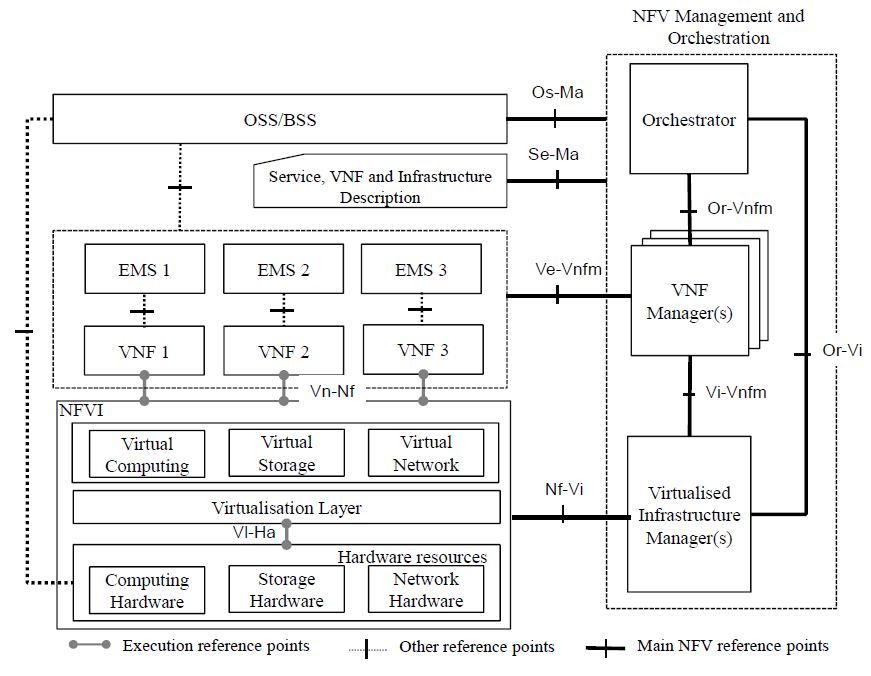
\includegraphics[width=0.95\textwidth]{nfv-mano}
	\caption{Архитектура NFV Management and Orchestration}
	\label{nfv-mano-image1}
\end{figure}

Каждый модуль обеспечивает определенный уровень абстракции. VIM занимается виртуализацией физических ресурсов. Менеджер функций предоставляет набор функций, размещенных на виртуальных ресурсах. Оркестратор управляет виртуальными сетевыми сервисами, которые построены на базе виртуальных сетевых функций.

Так же в архитектуре присутствуют неосновные модули:
\begin{itemize}
	\item описание виртуальных сетевых сервисов, функций и используемой ими инфраструктуры. В ETSI NFV MANO блоки, которые содержат такие описания, называют каталогами (catalog). В платформах, разрабатываемых на базе ETSI NFV MANO, функции каталогов обычно выполняют менеджеры соответствующего уровня (оркестратор сервисов, менеджер функций, VIM);
	\item система управления элементами (Element Management System, EMS). Система управляет работой элементов экземпляра виртуальной сетевой функции, отвечает за параметры функции. Данная система взаимодействует с менеджером функций через закрытые интерфейсы. Поэтому в существующих решениях, известных автору, данный модуль включен в состав менеджера функций.
\end{itemize}

Далее рассмотрим подробнее основные модули архитектуры ETSI NFV MANO.

\subsection{Менеджер виртуальной инфраструктуры}
Менеджер виртуальной инфраструктуры обеспечивает виртуализацию физической инфраструктуры в рамках одного домена. ETSI NFV MANO предполагает использование нескольких менеджеров инфраструктуры в одном домене. В задачи модуля входит:

\begin{itemize}
	\item управление полным жизненным циклом виртуальных ресурсов в рамках одного домена
	\begin{itemize}
		\item управление вычислительными ресурсами (computing resource) и хранилищами (storage);
		\item управление сетевыми ресурсами (networking resource), то есть управление коммутаторами, роутерами, сетевая настройка;
		\item остальные задачи гипервизора (асбтракция физической инфраструктуры, эффективное отображение ресурсов на их виртуальные аналоги и т.д.);
	\end{itemize}
	\item иметь полную информацию о доступных физических ресурсах и о запущенной виртуальной инфраструктуре;
	\item мониторинг за состоянием виртуальных ресурсов, обнаружение отказов оборудования, виртуальных машин, програмного обеспечения;
	\item оповещение остальных модулей о смене состояния виртуальной инфраструктуры;
	\item предоставление интерфейса для использования виртуальной инфраструктуры и для мониторинга физической инфраструктуры.
\end{itemize}

Подробнее о функциях VIM, и его спецификациях можно прочитать в стандарте \cite{nfv-mano-official-2016-04}.

\subsection{Менеджер виртуальных сетевых функций}
Менеджер виртуальных сетевых функций (VNFM) --- это основной модуль архитектуры ETSI NFV MANO, ответственный за  полный жизненный цикл виртуальных сетевых функций. Архитектура предполагает возможность наличиия нескольких менеджеров функций.

В ETSI NFV MANO следует отличать два понятия: описание виртуальной сетевой функции (VNF description) и экземпляр виртуальной сетевой функции (VNF instance). Когда говорят про сетевую функцию, чаще всего имеют ввиду ее спецификации, то есть ее описание. Экземпляр VNF --- это уже размещенная виртуальная инфраструктура, на которой функционирует программное обеспечение, присутствующее в описании функции. Таким образом, для каждой VNF существует единственное описание и множество ее экземпляров. Все экземпляры функции независимы друг от друга. В общем случае, они могут быть размещены в разных доменах (в разных VIM).

В задачи модуля входит:

\begin{itemize}
	\item регистрация и удаление VNF (в случае, если менеджер функций управляет сразу несколькими функциями);
	\item владение полной информации о спецификациях функции
	\begin{itemize}
		\item топология инфраструктуры, которую необходимо разместить для работы функции;
		\item входные параметры функции;
		\item исчерпывающая информация о программном обеспечении виртуальных машин;
		\item описание событий, по которым можно судить о состоянии функции (например, в ситуации, когда инфраструктура экземпляра функции недоступна, можно считать, что функция не работает)
		\item описание триггеров на вышеуказанные события (например, перезапустить виртуальную машину в случае, если она не отвечает на команду ping в течении 5 секунд)
	\end{itemize}
	\item управление жизненным циклом виртуальной функции
	\item отслеживание неисправностей в работе программного обеспечения функции;
	\item реакция на неисправности в работе VNF в соответствии с ее описанием (например, применить горизонтальное масштабирование в ответ на событие о недостатке производительности виртуальной машины);
	\item после размещения виртуальной инфраструктуры инициализировать ее, установить и настроить необходимое для работы функции программное обеспечение;
	\item обновление программного обеспечения уже размещенных виртуальных сетевых функций;
	\item оповещение остальных модулей о событиях, связанных с работой функции;
\end{itemize}

Более подробную спецификацию менеджера виртуальных функций можно посмотреть в стандарте \cite{nfv-mano-official-2016-04}.

\subsection{Оркестратор виртуальных сетевых сервисов}
Оркестратор виртуальных сетевых сервисов решает две основные задачи:
\begin{itemize}
	\item оркестрация ресурсов между несколькими менеджерами инфраструктуры, резервация ресурсов;
	\item управление жизненным циклом виртуальных сетевых сервисов;
\end{itemize}

Задача управления виртуальными сервисами нетривиальна. Она включает в себя множество подзадач:

\begin{itemize}
	\item предоставление интерфейса создания, удаления, изменения, обновления VNS;
	\item авторизация для управления сетевыми сервисами, разграничение прав доступа;
	\item синхронизация работы с менеджерами функций;
	\item отслеживание неисправностей в работе сервисов;
	\item реакция на события, связанные с изменением состояния сервиса;
	\item оповещение остальных модулей об изменении состояния сервисов;
	\item резервация ресурсов под сервисы с помощью модуля VIM;
\end{itemize}

Более подробный стандарт ETSI NFV MANO архитектуры NFV оркестратора находится в разработке, поэтому информацию о менеджере виртуальных сетевых сервисов можно получить, например, в высокоуровнем стандарте.\cite{nfv-mano-official-2016-04}





\chapter{Обзор существующих NFV платформ}
\label{nfv_platform_overview}
Рассмотрим существующие NFV платформы. Цель обзора -- выяснить достоинства и недостатки существующих решений и сформировать требования к разрабатываемому решению. Решения будут сравниваться по следующим критериям:
\begin{itemize}
	\item соответствие архитектуры платформы стандарту ETSI NFV MANO;
	\item независимость от платформы виртуализации ресурсов. Данный пункт означает, что решение использует программную прослойку (адаптер) для взаимодествия с платформой виртуализации. При необходимости перейте на другую платформу достачно заменить программную прослойку без переписывания кода основных модулей;
	\item поддержка работы с несколькими VIM одновременно. Решение, обладающее данным свойством, способно управлять несколькими платформами виртуализации ресурсов одновременно (один модуль VIM для одной платформы виртуализации);
	\item мониторинг состояния виртуального сетевого сервиса. Поддержка этого свойства позволяет следить за состоянием инфраструктуры виртуальных сетевых сервисов:
	\item автоматическое срабатывание триггеров scaling и healing. Scaling -- событие, связанное с масштабирование сервиса, healing -- событие, связанное с некорректной работой сервиса. Решение, в котором реализован данный пункт, может автоматически запускать триггеры на события scaling и healing, чтобы восстановить работу сервиса. Все триггеры заранее известны решению.
\end{itemize}

Выполнение всех критериев, указанных выше, позволит решению выполнять задачи по управлению виртуальными сетевыми сервисами и обеспечивать их отказоустойчивость и масштабируемость в автоматическом режиме.


\section{Open Platform for NFV}
Open Platform for NFV (OPNFV) - это платформа с открытым исходным кодом, на базе которой можно создавать компоненты  идеологии NFV. Проект OPNFV, используя архитектуру ETSI NFV MANO, фокусируется на разработке менеджера инфраструктуры (NFVI) архитектуры NFV MANO.\cite{opnfv-official}
Основные цели проекта:
\begin{itemize}
	\item разработка интегрированной и протестированной открытой платформы, которая сможет быть использована для построения NFV, ускорения внедрения новых продуктов и сервисов;
	\item привлечение заинтересованных лиц со стороны конечных заказчиков для удовлетворения требований пользовательского сообщества.
	\item создать экосистему NFV решений, основанную на открытых стандартах и программном обеспечении, удовлетворяющую требованиям конечных пользователей;
	\item продвигать OPNFV как предпочтительную платформу и сообщество для создания NFV решений с открытым кодом.
\end{itemize}

OPNFV стремится учавстовать в смежных открытых проектах, которые могут быть использованы в OPNFV, обеспечить целостность, производительность и функциональную совместимость компонентов. OPNFV активно взаимодействует с открытыми проектами: OpenStack, KVM, Open vSwitch, OpenDyalight, ONOS, Open Contrail, ETSI, IETF. Сообщество состоит из более чем 60 компаний, начиная с производителей оборудования и заканчивая поставщиками SDN и NFV решений.

Первый релиз (Arno) состоялся в июня 2015 году и какой-либо функциональности в себе не нес. Вторая версия проекта OPNFV (Brahmaputra) вышла 1 марта 2016 года. По словам сообщества, теперь платформа готова для проведения лабораторных тестов.\cite{opnfv-state1}

Как уже было отмечено, OPNFV - это база для реализации продуктов на базе NFV MANO. В данной платформе разрабатывается лишь модуль NFVI, отвечающий за виртуальные ресурсы. Задачи по масштабируемости и отказоустойчивости здесь выполняются только на уровне виртуальных и физических ресурсов.


\section{Cloudify}
Cloudify - это платформа с открытым исходным кодом. Cloudify архитектурно состоит из основного модуля, называемого Cloudify Manager VM, и Cloudify агентов, установленных на подконтрольных виртуальных машинах. 

Cloudify Manager VM исполняет роли сразу двух основных модулей - это VNFM и NFVO. Таким образом, указанный модуль выполняет множество задач:
\begin{itemize}
	\item регистрация новых виртуальных функций. Описание функций представляется в формате собтсвенной разработки, называемый blueprints. Он основан на стандарте описания функций TOSCA (формат, основанный на YAML);
	\item размещение инфраструктуры VNF, используя плагины к существующим платформам виртуализации ресурсов (поддерживаются Openstack, VMware);
	\item инициализация инфраструктуры функций, использую программы-агенты на подконтрольных виртуальаных машинах;
	\item мониторинг изменения состояния виртуальных функций с помощью агентов;
	\item запуск триггеров из описания функции;
\end{itemize}

Cloudify агенты ответственны за выполнения команд Cloudify Manager VM. Различают агентов со стороны Cloudify менеджера (manager side agents) и со стороны виртуальной сетевой функции (application side agents). Агенты менеджера устанавливаются вместе с операционной системой виртуальной машины и выполняют следующие служебные задачи: создание виртуальной машины, привязка внешнего ip-адреса и т.д.. Агенты виртуальной функции являются опцией (устанавливаются, если стоит соответствующая запись в описании функции). Задачи, выполняемые агентами фукнции, должны присутствовать в описании функции.\cite{cloudify-official-oveview1}

Изучение платформы Cloudify показало, что в действительности полной автоматизации процесса мониторинга и срабатывание триггеров еще не достигнуто. После размещения функции требуется часть настроек произвести в ручном режиме. 


\section{OpenStack Tacker}
Openstack Tacker - это проект с открытым исходным кодом. Использует разработки проекта OPNFV. Основной целью проекта является реализация основных блоков ETSI NFV MANO (VNF-Manager и VNF-Orchestrator) в виде плагина для платформы облачной виртуализации Openstack. Tacker реализует управление виртуальными функциями и оркестрацию сетевых сервисов.
	Рассмотрим основную функциональность базовых блоков архитектуры ETSI NFV MANO в рамках проекта Tacker. Основные задачи, выполняемые блоком VNF-Manager:
\begin{itemize}
	\item хранилище всех виртуальных функций, доступных системе;
	\item управление полным жизненным циклом каждой виртуальной функции (размещение, инициализация, масштабирование, остановка, удаление);
	\item мониторинг за размещенными виртуальными функциями. Основные параметры мониторинга: производительность и отказоустойчивасть работы функции;
	\item автоматическое восстановление работы функции в случае ее полного или частичного отказа в предоставлении услуги по заданным политикам;
	\item облегчение первоначальной настройки виртуальной сетевой функции;
\end{itemize}
Задачи, выполняемые блоком VNF-Orchestrator:
\begin{itemize}
	\item использования шаблонов при управлении сетевыми сервисами, комбинируя различные виртуальные функции между собой;
	\item обеспечение эффективного размещения виртуальных функций;
	\item создание цепочек виртуальных сетевых функций (сетевые сервисы);
	\item контроль за выделение ресурсов с помощью блока VIM;
	\item оркестрация виртуальных функций на множестве различных блоков VIM.
\end{itemize}

На текущий момент возможности Tacker реализованы только командном интерфейсе и не доступны в графическом интерфейсе Horizon платформы Openstack.\cite{tacker-official} 
Восстановление работы функции и расширение инфраструктуры функции доступно только в ручном режиме.


\section{OpenBaton}
OpenBaton - проект с открытым исходным кодом, реализующий архитектуру ETSI NFV MANO. Основными модулями платформы являются:
\begin{itemize}
	\item оркестратор сетевых сервисов NFVO;
	\item менеджер виртуальных сетевых функций VNFM;
\end{itemize}

Основным модулем, над которым ведется разработка - это NFVO. В нем содержится основная функциональность по размещению функций, слежению за их состоянием, восстановлению из аварийного состояния и масштабированию. VNFM - является заменяемым модулем: возможно использование модуля управления функциями собственной разработки. При этом с OpenBaton поставляются библиотеки, позволяющие упростить разработку и интегрирование собственного VNFM с оркестратором.

OpenBaton независима от платформы виртуализации ресурсов. На текущий момент разработан только плагин под плафторму Openstack. Разработчиками заявлена поддержка нескольких VIM. В OpenBaton для включения функции мониторинга необходимо дополнительно установить Zabbix сервер (о поддержке других решений по слежению за виртуальными машинами автору не известно).

На момент написания работы в OpenBaton идет разработка следующей функциональности: развертывания дополнительной инфраструктуры и разнообразные улучшения в blueprints. Из этого следует, что о реализации автоматического масштабирования и восстановления функции речи пока не идет.

Для реализации собственных виртуальных сетевых сервисов OpenBaton предлагает либо реализовать менеджер функций собственной разработки, либо привести описании функции через VNFPackage. VNFPackage - это описание функции на основе формата YAML, который содержит необходимое описание виртуальной функции.\cite{bib:openbaton-official}


\section{Проприетарные решения}
Автору не известны проприетарные решения, реализующие концепцию NFV. Наиболее популярные продукты Microsoft Azure и VMware vSphere работают в рамках модели IaaS (Infrastructure as as Service, инфраструктура как услуга). Указанные платформы можно использовать только в качестве менеджера инфраструктуры в рамках ETSI NFV MANO.





\chapter{Исследование и построение решения задачи}
\section{Анализ результатов обзора}
Результаты обзора, приведенные в таблице \ref{tab:nfv_platform_comprassion}, показали, что ни одно из существующих решений полностью не удовлетворяет установленным требованиям.

\renewcommand{\arraystretch}{1.5}
\begin{table}[h]
\center % центрирование таблицы
\begin{tabular}{|p{0.2\textwidth}|p{0.1\textwidth}|p{0.125\textwidth}|p{0.125\textwidth}|p{0.125\textwidth}|p{0.125\textwidth}|} % разделить колонки вертикальными линиями и центрировать содержимое каждой колонки
\hline % прочертить горизонтальную линию
Плат\-фор\-ма & ETSI NFV MANO & Не\-за\-ви\-си\-мость от платформы виртуализации ресурсов & Од\-но\-вре\-мен\-ная работа с несколькими VIM & Мо\-ни\-то\-ринг состояния VNS & ав\-то\-ма\-ти\-чес\-кое срабатывание триггеров scaling, healing \\
\hline
OPNFV & + & + & - & ? & ? \\
\hline
Cloudify & + & + & ? & + & - \\
\hline
Openstack Tacker & + & - & - & ? & ? \\
\hline
%CORD on.lab & & & & & \\
%\hline
OpenBaton & + & + & + & + & - \\
\hline
%vSphere & ? & ? & ? & ? & ? \\
%\hline
%Azure & ? & ? & ? & ? & ? \\
%\hline
\end{tabular}
\caption{Сравнение существующих NFV решений.}
\label{tab:nfv_platform_comprassion}
\end{table}


\section{Требования к решению}
В результате анализа существующих NFV платформ сформируем требования к разрабатываемому решению:
\begin{enumerate}
	\item по запросу осуществлять подписку и отписку пользователей от виртуальных сетевых сервисов в рамках модели Software as a Service (SaaS);
	\item при возникновении неисправности принимать меры по восстановлению корректной работы сервиса в автоматическом режиме (healing);
	\item обеспечивать масштабируемость инфраструктуры сервиса в автоматическом режиме (scaling);
	\item решение должно быть независимым от платформы виртуализации инфраструктуры;
	\item решение должно быть согласовано с высокоуровневой архитектуры ETSI NFV MANO;
	\item поддержка нескольких плафторм виртуализации инфраструктуры одновременно;
\end{enumerate}


\section{План построения решения задачи}
\label{section-platform-requirements}
Прежде чем перейти непосредственно к решению задачи необходимо понять, какие модули архитектуры ETSI NFV MANO относятся к установленным требованиям.

Оркестратор сетевых сервисов согласно ETSI NFV MANO занимается:
\begin{itemize}
	\item подпиской и отпиской пользователей от сервиса;
	\item масштабируемостью инфраструктуры сервиса (scaling) в автоматическом режиме;
	\item восстановлением корректной работы сервиса при возникновении неисправности (healing) в автоматическом режиме.
\end{itemize}

Поддержка нескольких модулей VIM также решается на уровне оркестратора. Независимость от платформы виртуализации решается на уровне менеджера инфраструктуры (этот модуль должен использовать плагин для работы с конкретной платформой виртуализации ресурсов).

Таким образом, для решения поставленной задачи достаточно:
\begin{enumerate}
	\item реализовать оркестратор сетевых сервисов (NFVO) согласно архитектуры ETSI NFV MANO;
	\item внедрить оркестратор в платформу, удовлетворяющую следующим требованиям:
	\begin{itemize}
		\item плафторма обеспечивает виртуализацию ресурсов;
		\item платформы обладает средствами мониторинга для слежения за виртуальными машинами и связующими их каналами.
	\end{itemize}
\end{enumerate}





\chapter{Описание практической части}
\label{chap:practice}
В текущей главе приведено описание реализации модуля VNF-O плафтормы Cloud Conductor. В результате реализации такого модуля платформа будет полностью удовлетворять требованиям, описанным в разделе \ref{section-platform-requirements}. Проект разрабатывается в отечественной организации Центр Прикладных Исследований Компьютерных Сетей (ЦПИКС).

\section{Облачная платформа Cloud Conductor}
Рассматриваемая облачная платформа ориентирована на предоставление услуг по модели IaaS (). Основной задачей проекта - управление несколькими платформами виртуализации ресурсов (в частности Openstack). Взаимодействие между внутренними модулями оуществляется через библиотеку RabbitMQ (RMQ).

Проект Cloud Conductor состоит из нескольких модулей:
\begin{itemize}
	\item GUI-client;
	\item GUI-server;
	\item модуль виртуализации инфраструктуры (VIM);
	\item модуль мониторинга Monitoring (Mon);
	\item менеджер функций (VNF-M, в разработке);
	\item менеджер сервисов (VNF-O, в разработке);
\end{itemize}

Далее более подробно будут рассмотрены уже разработанные модули

\subsection{Графический интерфейс}
Оба модуля (GUI-client и GUI-server) отвечают за:
\begin{itemize}
	\item отображение актуальной информации о текущей загрузке физических серверов;
	\item отображения размещенных тенантов;
	\item авторизацию пользователей;
	\item предоставление управления виртуальными сетевыми функциями и виртуальными сетевыми сервисами (в разработке);
	\item отображение актуального состояния сетевых функций и сервисов (в разработке).
\end{itemize}

Модуль GUI-server будет использовать интерфейс модуля VNF-O для отображения и управления виртуальными сетевыми функциями и сервисами.

\subsection{Модуль виртуализации ресурсов}
Модуль состоит из двух основных частей: плагин для существующей платформы виртуализации ресурсов (используется Openstack) и независимая часть для обработки сообщений от других модулей проекта Cloud Conductor (Mon, VNF-M, GUI-server и т.д.). Плагин может изменяться в зависимости от платформы виртуализации ресурсов (Openstack, VMWare и т.д.). Задача второй части заключается в управлении тенантами (сеть с виртуальными машинами) по запросу от других модулей проекта. 

Основные интерфейсы для других модулей: размещение и удаление тенанта, предоставление консоли к конкретной виртуальной машине, предоставление информации о размещенных сетях и виртуальных машинах, информация о занятых ресурсах и т.д..

\subsection{Модуль мониторинга}
Модуль мониторинга так же состоит из двух частей: плагин для существующей программы мониторинга (используется Zabbix) и независимая часть для обработки сообщений от других модулей проекта Cloud Conductor (GUI-server, VNF-M, и т.д.). Плагин может изменяться в зависимости от программы мониторинга. Независимая часть обеспечивает слежение за виртуальными машинами, соединениями между ними.

Основные интерфейсы для других модулей: установка и удаление мониторов за виртуальными машинами, оповещение подписанных модулей о событиях, предоставление статистики по работе виртуальных машин.

\subsection{Модуль управления виртуальными сетевыми функциями}
Модуль управления виртуальными сетевыми функциями состоит из двух основных частей: часть для анализа описания виртуальных сетевых функций и часть для взаимодействия с другими модулями проекта Cloud Conductor (VNF-O, VNF-M). Модуль умеет регистрировать виртуальную сетевую функцию, внося соответствующую информацию в базу данных. Модуль, анализируя описание фукнции занимается конфигурацией инфраструктуры для работы функции.

Основной интерфейс, предоставляемый модулю VNF-O: управление, конфигурирование и поддержка виртуальных сетевых функций.


\section{Описание реализованного модуля}
Модуль состоит из следующих основных классов:
\begin{itemize}
	\item VNFOrchestrator -- класс, инициализирующий все остальные части программы (обработчики сообщений, базу данных, логгирование и т.д.).
	\item менеджеры сообщений, взаимодействующими с другими модулями платформы:
	\begin{itemize}
		\item GUIManager -- класс, обрабатывающий запросы от модуля GUI;
		\item MonitoringManager -- класс для отправки запросов на добавление и удаление мониторов за виртуальными машинами и для обработки событий, связанных с функционированием виртуальных машин;
		\item VIMManager -- класс, отправляющий запросы для управления инфраструктурой сети виртуальных машин;
		\item VNFManager -- класс, отправляющий запросы для управления виртуальными сетевыми функциями и обрабатывающий запросы на изменение инфраструктуры конкретной виртуальной функции;
	\end{itemize}
	\item DataBase -- класс, отвечающий за взаимодействие с базой данных (БД). Реализует соединение с БДи предоставление сессии для взаимодействия. В качестве БД используется MySQL;
	\item Messenger -- класс, обобщающий взаимодействие между модулями платформы. Занимается отправкой и приемом сообщений используя адаптеры для библиотеки RabbitMQ:
	\begin{itemize}
		\item RabbitMQConsumer -- адаптер для приема сообщений через библиотеку RabbitMQ;
		\item RabbitMQPublisher -- адаптер для отправки сообщений через библиотеку RabbitMQ;
	\end{itemize}
\end{itemize}
Как было сказано выше, в рамках данной работы разрабатывался модуль, соответствующий уровню оркестратора сетевых сервисов в архитектуре ETSI NFV MANO. 
На рисунке \ref{pic:classes_diagram} можно увидеть диаграмму классов разработанного модуля.
\begin{figure}[h]
	\centering
	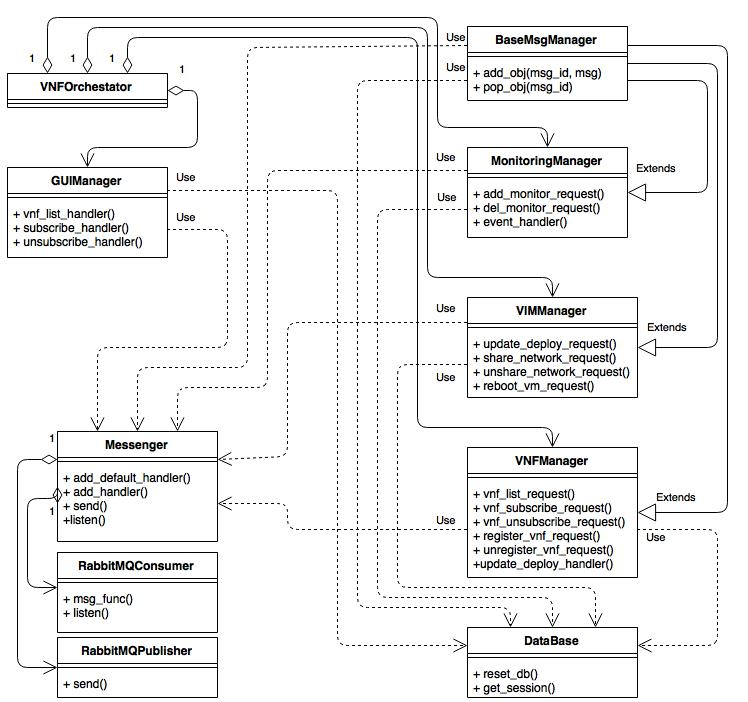
\includegraphics[width=0.95\textwidth]{classes_diagram}
	\caption{Диаграмма классов модуля реализованного модуля}
	\label{pic:classes_diagram}
\end{figure}

Рассмотрим схему взаимодействия классов разработанного модуля на примере подписке клиента на виртуальный сетевой сервис. Подписка клиента осуществляется через серию шагов:
\begin{enumerate}
	\item GUIManager получает запрос на подписку виртуальный сетевой сервис и начинает его обработку (subscribe\_handler);
	\item GUIManager с помощью VNFManager запрашивает подписку на каждую виртуальную сетевую функцию, содержащуюся в сервисе (vnf\_subscribe\_request);
	\item в результате предыдущего запроса модуль управления виртуальными сетевыми функциями должен запросить разместить инфраструктуру для каждой функции. Для этого он обращается к разработанному модулю с соответствующим запросом, который обрабатывает VNFManager (update\_deploy\_handler);
	\item VNFManager выполняет запрос на обновлении инфраструктуры, используя VIMManager (update\_deploy\_request);
	\item после успешного выполнения предыдущего запроса VNFManager передает информацию о размещенной инфраструктуре в модуль управления виртуальными сетевыми функциями;
	\item модуль управления функциями сообщает об успешно произведенной настройке всех виртуальных функций, входящих в состав сервиса.
	\item GUIManager с помощью MonitoringManager устанавливает мониторы за размещенными виртуальными машинами (add\_monitor). 
	\item GUIManager с помощью VIMManager соединяет виртуальную машину клиента с инфраструктурой виртуального сетевого сервиса (share\_network);
	\item после успешной подписки клиента к сервису GUIManager сообщает модулю GUI об успешной подписке клиента
\end{enumerate}




\chapter{Экспериментальные исследования}
\label{chap:expirements}
В качестве доказательства выполнения требований 2 и 3 из раздела \ref{chap:problem_statement} проведем эксперименты healing и scaling, в которых покажем автоматическое восстановление работы сервиса и автоматическое расширение инфраструктуры сервиса соответственно.

\section{Эксперимент healing}
\subsection{Описание эксперимента}
Во время использование клиентом виртуального сетевого сервиса происходит отказ в инфраструктуре функции. Оркестратор должен восстановить работу сервиса.

\subsection{Входные данные}
\begin{itemize}
	\item зарегистрированна виртуальная функция proxy в менеджере функций;
	\item зарегистрирован виртуальной сетевой сервис прокси, состоящий из одной функции proxy;
	\item размещена виртуальная машина клиента в облаке (напомним, что плафторму Cloud Conductor позволяет размещать виртуальные машины клиентов в своем облаке);
	\item виртуальная машина клиента подключена к сервису прокси.
\end{itemize}

\subsection{Ожидаемая реакция}
В результате недоступности одной из виртуальных машин, модуль мониторинга генерирует событие, соответствующее отказу соединения между виртуальной машиной клиента и экземпляром сервиса, и отправляет его оркестратору сетевых сервисов. Оркестратор, получив событие об отсутствии соединения между клиентом и сервисом, решает перезапустить неправильно работающие сетвые интерфейсы виртуальных машин. Таких интерфейсов два: у виртуальной машины клиента и у виртуальной машины сетевой функции. Запрос не перезапуск интерфейсов отправляется в менеджер инфраструктуры. После получение ответа о успешном перезапуске интерфейсов оркестратором клиент продолжает потреблять сервис.

\subsection{Результаты эксперимента}
TODO

\section{Эксперимент scaling}
\subsection{Описание эксперимента}
В результате высокой нагрузки инфраструктура сервиса оказывается перегружена. Поэтому клиенты испытывают дискомфорт при потреблении сервиса (задержки). Оркестратор должен увеличить объем ресурсов, выделяемых для работы сервиса, чтобы исправить ситуацию.

\subsection{Входные данные}
\begin{itemize}
	\item оркестратор работает с двумя менеджерами инфраструктуры, каждый из которых управляет ресурсами подконтрольного ему центра обработки данных (ЦОД).
	\item зарегистрирована виртуальная функция proxy в менеджере функций;
	\item зарегистрирован виртуальной сетевой сервис прокси, состоящий из одной функции proxy;
	\item размещена виртуальная машина клиента в облаке;
	\item экземпляр функции, использующийся клиентом, размещен на первом ЦОД;
	\item виртуальная машина клиента подключена к сервису прокси.
\end{itemize}

\subsection{Ожидаемая реакция}
При обнаружении перегрузки одной из виртуальных машин сервиса, модуль мониторинга генерирует соответствующее событие и отправляет его менеджеру функций. Получив событие о некорректной работе виртуальной машины из функции proxy, менеджер считывает описание функции. Согласно описанию менеджер делает запрос в оркестратор на расширение ифнраструктуры сервисного тенанта. Оркестратор оценивает запрос менеджера на инфраструктуру и оставшийся запас ресурсов в первом ЦОД. Ресурсов в первом ЦОД оказывается недостаточно, но во втором ЦОД их хватает для удовлетворения запроса. Поэтому оркестратор решает переместить тенант с функцией с первого ЦОД на второй. После получения ответа об успешном размещение функции клиент продолжает потреблять сервис.

\subsection{Результаты эксперимента}
TODO





\chapter*{Заключение}
\addcontentsline{toc}{chapter}{Заключение} % добавить Заключение в оглавление
Обзор существующих платформ виртуализации сервисов показал, что ни одно из существующих решений не удовлетворяет поставленной задаче. В рамках данной работы был разработан модуль для платформы Cloud Conductor, позволяющий автоматизировать процессы восстановления и расширения сетевых сервисов. Решение позволяет осуществлять управление подключением пользователей к сервисам. 





% Список литературы
\begin{thebibliography}{00}
\bibitem{nfv-mano-official-2016-04} Network Functions Virtualisation (NFV); Management and Orchestration. URL: http://www.etsi.org/deliver/etsi\_gs/NFV-MAN/001\_099/001/01.01.01\_60/gs\_NFV-MAN001v010101p.pdf (дата обращения 01.04.2016)
\bibitem{nfv-mano-state1} ETSI NFV Management and Orchestration (MANO) простым языком. URL: https://sdnblog.ru/etsi-nfv-mano-beginners-tutorial/ (дата обращения 01.04.2016)
\bibitem{nfv-official} Network Functions Virtualisation (NFV); use cases. URL: http://www.etsi.org/technologies-clusters/technologies/nfv (дата обращения 01.04.2016)
\bibitem{nfv-state2} NFV для корпоративных сервисов - № 12, 2014. URL: http://www.osp.ru/lan/2014/12/13044225 (дата обращения 01.04.2016)
\bibitem{nfv-state1} NFV виртуализация сетевых функций. URL: http://sci-article.ru/stat.php?i=1455156066 (дата обращения 01.04.2016)
\bibitem{opnfv-official} Open Platform for NFV (OPNFV). URL: https://www.opnfv.org (дата обращения 01.04.2016)
\bibitem{opnfv-state1} Чем занимается сообщество OPNFV? URL:  https://sdnblog.ru/who-is-opnfv/ (01.04.2016)
\bibitem{cloudify-official-oveview1} Cloudify Overwiew. URL: http://getcloudify.org/guide/3.1/overview-architecture.html (дата обращения 01.04.2016)
\bibitem{tacker-official} Tacker. URL: https://wiki.opfirewallenstack.org/wiki/Tacker (дата обращения 01.04.2016)
\bibitem{bib:openbaton-official} OpenBaton. URL: http://openbaton.github.io/ (дата обращения 01.04.2016)
\bibitem{bib:saas} Модель SaaS в мире и в России. URL: http://www.bytemag.ru/articles/detail.php?ID=12825 (дата обращения 01.04.2016)
\end{thebibliography}

% Конец документа
\end{document}


